
\chapter{Timing and Bandwidth Calculation}
\label{chap:Timing_Bandwidth}
%\label{sec:timing-bandw-calc}

\section{Timing}
\label{sec:timing}

We can use either CPU timers or GPU timers. To use CPU timers, we need
to  add \verb!cudaThreadSynchronize()! immediately before starting
and stopping CPU timer to accurately measure the time. 
However, there are certain restrictions when using CPU timers

\begin{enumerate}
\item Only suitable for timing code in the default stream (stream
  0). The reason is that the driver may interleave execution of CUDA
  calls from non-default streams; thus the calls to these streams may
  be included in the timing of a non-default-stream kernel.

  It means that default stream exhibit synchronous behavior, i.e. an
  operation in the default stream can begin only after all preceding
  calls in any stream have completed; and when it starts, no
  subsequent operations in any stream can begin until it finishes. 
\end{enumerate}

To use GPU timers, you need to create two CUDA events, record the time
difference between the two events (in miliseconds and a resolution of
approximately half a microsecond).

\begin{lstlisting}
cudaEvent_t start, stop;
float time;

cudaEventCreate(&start);
cudaEventCreate(&stop);

cudaEventRecord( start, 0);
kernel<<<grid, threads>>> (d_odata, d_idata, size_x, size_y,
NUM_REPS);

cudaEventRecord( stop, 0);
cudaEventSynchronize( stop);

cudaEventElapsedTime( &time, start, stop);
cudaEventDestroy( start);
cudaEventDestroy( stop);
\end{lstlisting}

To put the event into the default stream, we use
\verb!cudaEventRecord! with the stream ID is the second argument. To
tell the time difference between two events, you use
\verb!cudaEventElapsedTime!. The measurement use GPU clocks, so it is
OS-independent.

\section{Bandwidth (GPU-device memory)}
\label{sec:bandwidth}

The theoretical bandwidth between device memory and the GPU is
computed as follows, e.g. 
\begin{itemize}
\item GeForce GTX 280
  \begin{equation*}
    (1107 \times 10^6 \times (512/8) \times 2 ) / 10^9 = 141.6 \text{ GB/sec}
  \end{equation*}
  with 1107 MHz is the memory clock rate, 512-bit wide memory interface
  (divided by 8 to convert to byte), double data rate (multiply by 2);
  and divided by $10^9$ to convert to GB/sec (GBps). 

\item G80 chips
  \begin{equation*}
    (900 \times 10^6 \times (384/8) \times 2) / 10^9 = 86.4 \text{ GB/sec}
  \end{equation*}
  with 384-bit memory interface running in 900 MHz double-data rate.
\end{itemize}


Some calculation use $1024^3$, rather than $10^9$, then the result
would be 131.9 GBps. You can use either one, but make sure you use the
same value when calculating {\bf effective bandwidth} so that the
comparison is valid. 

\begin{equation*}
  \text{Effective bandwidth} = ((B_r + B_w)/10^9) / \text{ time}  [GBps]
\end{equation*}
with $B_r$ is the number of bytes read, and $B_w$ is the number of
bytes write per kernel; and \verb!time! is given in seconds. Again,
you can use either $10^9$ or $1024^3$.

Example: A 2048x2048 float matrix copy has the effective bandwidth
\begin{equation*}
  \text{Effective bandwidth} = ((4\times 2048^2 + 4\times 2048^2)/10^9) / \text{ time}  [GBps]
\end{equation*}

TRICK: Comment out the arithmetic operations if you want to assess
memory-only performance which is fine as long as memory access is not
data-dependent.


\section{Memory Throughput reported by cudaprof}
\label{sec:thro-report-cudapr}

The throughput reported is measured by using some SMs and then
extrapolated to the whole chip, thus it is an estimate of data
throughput. Normally, this value is greater than the {\it effective
  bandwidth}. So, for publication purpose, you should use effective
bandwidth. However, throughput reported by cudaprof is a good estimate
of how much bandwidth is wasted. 

Memory throughput is the bottle neck of many applications. So, when
coding from scratch, you should start with memory operation first to
achieve a good throughput.
\begin{enumerate}
\item 70-80\% to the theoretical bandwidth is very good, 
\item 50\% to the theoretical bandwidth is good in non-trivial
  arithmetic (e.g. exponential, trigonometric operations...)
\end{enumerate}
You can measure memory throughput 
\begin{enumerate}
\item from the app point of view, i.e. ``useful'' bytes
\item from the hardware point of view, i.e. actual bytes moved across
  the bus. 
\end{enumerate}

CUDA Visual profiler will give you the information from the hardware
point of view, Fig.~\ref{fig:cudaprof}. 
\begin{itemize}
\item It counts the number of 32-byte, 64-byte and 128-byte segment
  transaction on the TPC. Then it extrapolate from one TPC to the
  entire GPU by multiplying by (total threadblocks / threadblocks per
  TPC) or (grid size / cta launched). 

  NOTE: 
  \begin{itemize}
  \item cta launched = Cooperative Thread Array (thread block)
    launched, i.e. the number of thread blocks run on TPC 0 (NOT
    available in Fermi as there is no TPC concept in Fermi).
  \item sm cta launched = number of thread blocks run on SM 0.
  \end{itemize}
\item 
\end{itemize}

\begin{figure}[hbt]
  \centerline{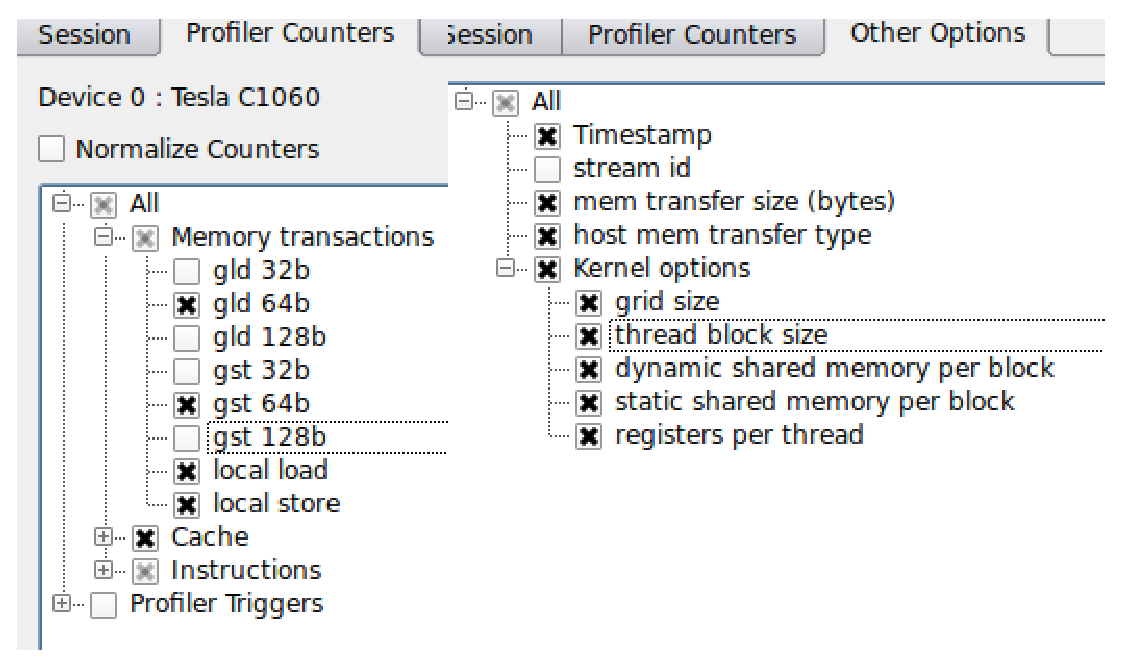
\includegraphics[height=5cm,
    angle=0]{./images/cudaprof_check.eps}}
  \caption{What should be enabled in cudaprof}
  \label{fig:cudaprof}
\end{figure}

The theory (peak) throughput is
\begin{enumerate}
\item Fermi: 
  \begin{itemize}
  \item Shared memory: 1030 GB/s aggregate
  \item L1: 1030 GB/s
  \item L2: 230 GB/s (not affected by ECC)
  \item DRAM: 144 GB/s (115 GB/s with ECC)
  \end{itemize}
\end{enumerate}

\section{Instruction throughput}
\label{sec:instr-thro-flow}

To process an instruction in a warp of threads, a multiprocessor (SM)
must
\begin{enumerate}
\item read the instruction operands for each thread in the warp,
  i.e. fetch the data (this may have high latency if the data is in
  off-chip memory)
\item execute the instruction
\item write the result for each thread of the warp
\end{enumerate}
So, the instruction throughput depends on (and is maximized if)
\begin{enumerate}
\item the nominal instruction throughput (minimized the use of low
  throughput instructions), read
  Sect.~\ref{sec:warp-sched-latency-1}. 

\item memory latency and bandwidth (maximize the use of available
  bandwidth for each category of memory)
\item memory access pattern (avoid shared memory bank conflict, try to
  access in contiguous memory)
\item thread scheduler to overlap memory transaction with mathematical
  computation (as much as possible, i.e. high number of arithmetic
  operations per memory operation, and many active threads)
\end{enumerate}

Functions with \verb!__! prefix, i.e. \verb!__func()! map directly to
the hardware ISA. E.g. \verb!__sin(x)!, \verb!__exp(x)!,
\verb!__pow(x,y)!. Otherwise, i.e. \verb!func()! are compiled to
multiple instructions which run slower but have higher accuracy
(i.e. 5 ulp or less). E.g. sin(x), epx(x), pow(x,y)

There are additional intrinsic functions with explicit IEEE rounding
mode (rz, rn, ru, rd), e.g. \verb!__sincosf()!, \verb!__frcp_rz()!...


The profiler tell the instruction throughput is based on fraction of
\verb!fp32! arithmetic operations that could be issued at the same
amount of time. So, it's not a good metric with \verb!fp64! arithmetic
or transcendental operations in CUDA Visual Profiler.


The data is computed from one SM and extrapolated to whole GPU chip. 
The theory (peak) throughput is
\begin{enumerate}
\item Fermi: 
  \begin{itemize}
  \item FP32: 1030 GFLOPS/s 
  \item FP64: 515 GFLOPS/s
  \end{itemize}
\end{enumerate}

\begin{framed}
  The perfect balance between instructions : gmem bytes is
  \verb!3.5:1! (or \verb!4.5:1! if ECC is on). If you have a higher
  ratio, then the program is instruction bound, otherwise, it is
  memory bound. 
\end{framed}


TRICK: You can comment out \verb!gmem! access to assess
arithmetic-only performance, which is fine as long as computation is
not data dependent. However, noting that eliminating reads is
straightforward, yet not with eliminating writes. The reason is that
the compiler with throw away all code it deems as not contributing to
output. To workaround, we can precede write with an IF statement that
always fails, e.g.
\begin{lstlisting}
if (threadIdx.x == -2) { ...} 
\end{lstlisting}

\section{Control flow}
\label{sec:control-flow}

As instructions are issued per 32 threads (i.e. a warp), it's
important for threads in a group to execute the same instruction to
achieve the optimal performance. Divergent may occur when IF-ELSE
construct are used in the kernels. 

As threads in different warps can execute different code with no
impact on the performance, as long as threads in the same warp execute
the same instruction; we can use the \verb!WARP_SIZE! to determine the
branching. 

{\bf Example}: no divergence. We call {\it branch granularity is a
  whole multiple of warp size}
\begin{lstlisting}
IF (threadIdx.x / WARP_SIZE > 2) { ...} ELSE {... }
\end{lstlisting}

{\bf Example}: with divergence, e.g. threads in the first warp are
divergent. We call {\it branch granularity is smaller than warp size}
\begin{lstlisting}
IF (threadIdx.x > 2) {...} ELSE {...}
\end{lstlisting}

The profiler can tell
\begin{enumerate}
\item number of divergent branches
\item warp serialization
\item how many instructions are issued 
\end{enumerate}

\section{Bandwidth (device memory-host memory)}
\label{sec:bandw-device-memory}

The peak bandwidth between host memory and device memory on PCIe
$\times 16$ Gen 2 cards are 8 GBps. It's recommended using
{\it pinned} (page-locked) memory for regularly data transfer, e.g. on
PCIe $\times 16$ Gen2 cards, it can reach the peak 5GBps transfer
rates.


\section{Benchmarks}
\label{sec:benchmarks}

To keep a GPU running, so that we don't have to wait for it to
warm-up, we need to have \verb!pgcudainit! to run in the background. 

\subsection{A cluster}
\label{sec:cluster-1}

To benchmark in a cluster, we can use Network Protocol Independent
Performance Emulator (netPIPE).




\subsection{Latency and throughput of memory transfer}
\label{sec:latency-thro-memory}

To measure the latency and throughput of memory transfer in a cluster
based on the principle of HINT benchmark, we use Network Protocol
Independent Performance Emulator (NetPIPE).

\begin{figure}[hbt]
  \centerline{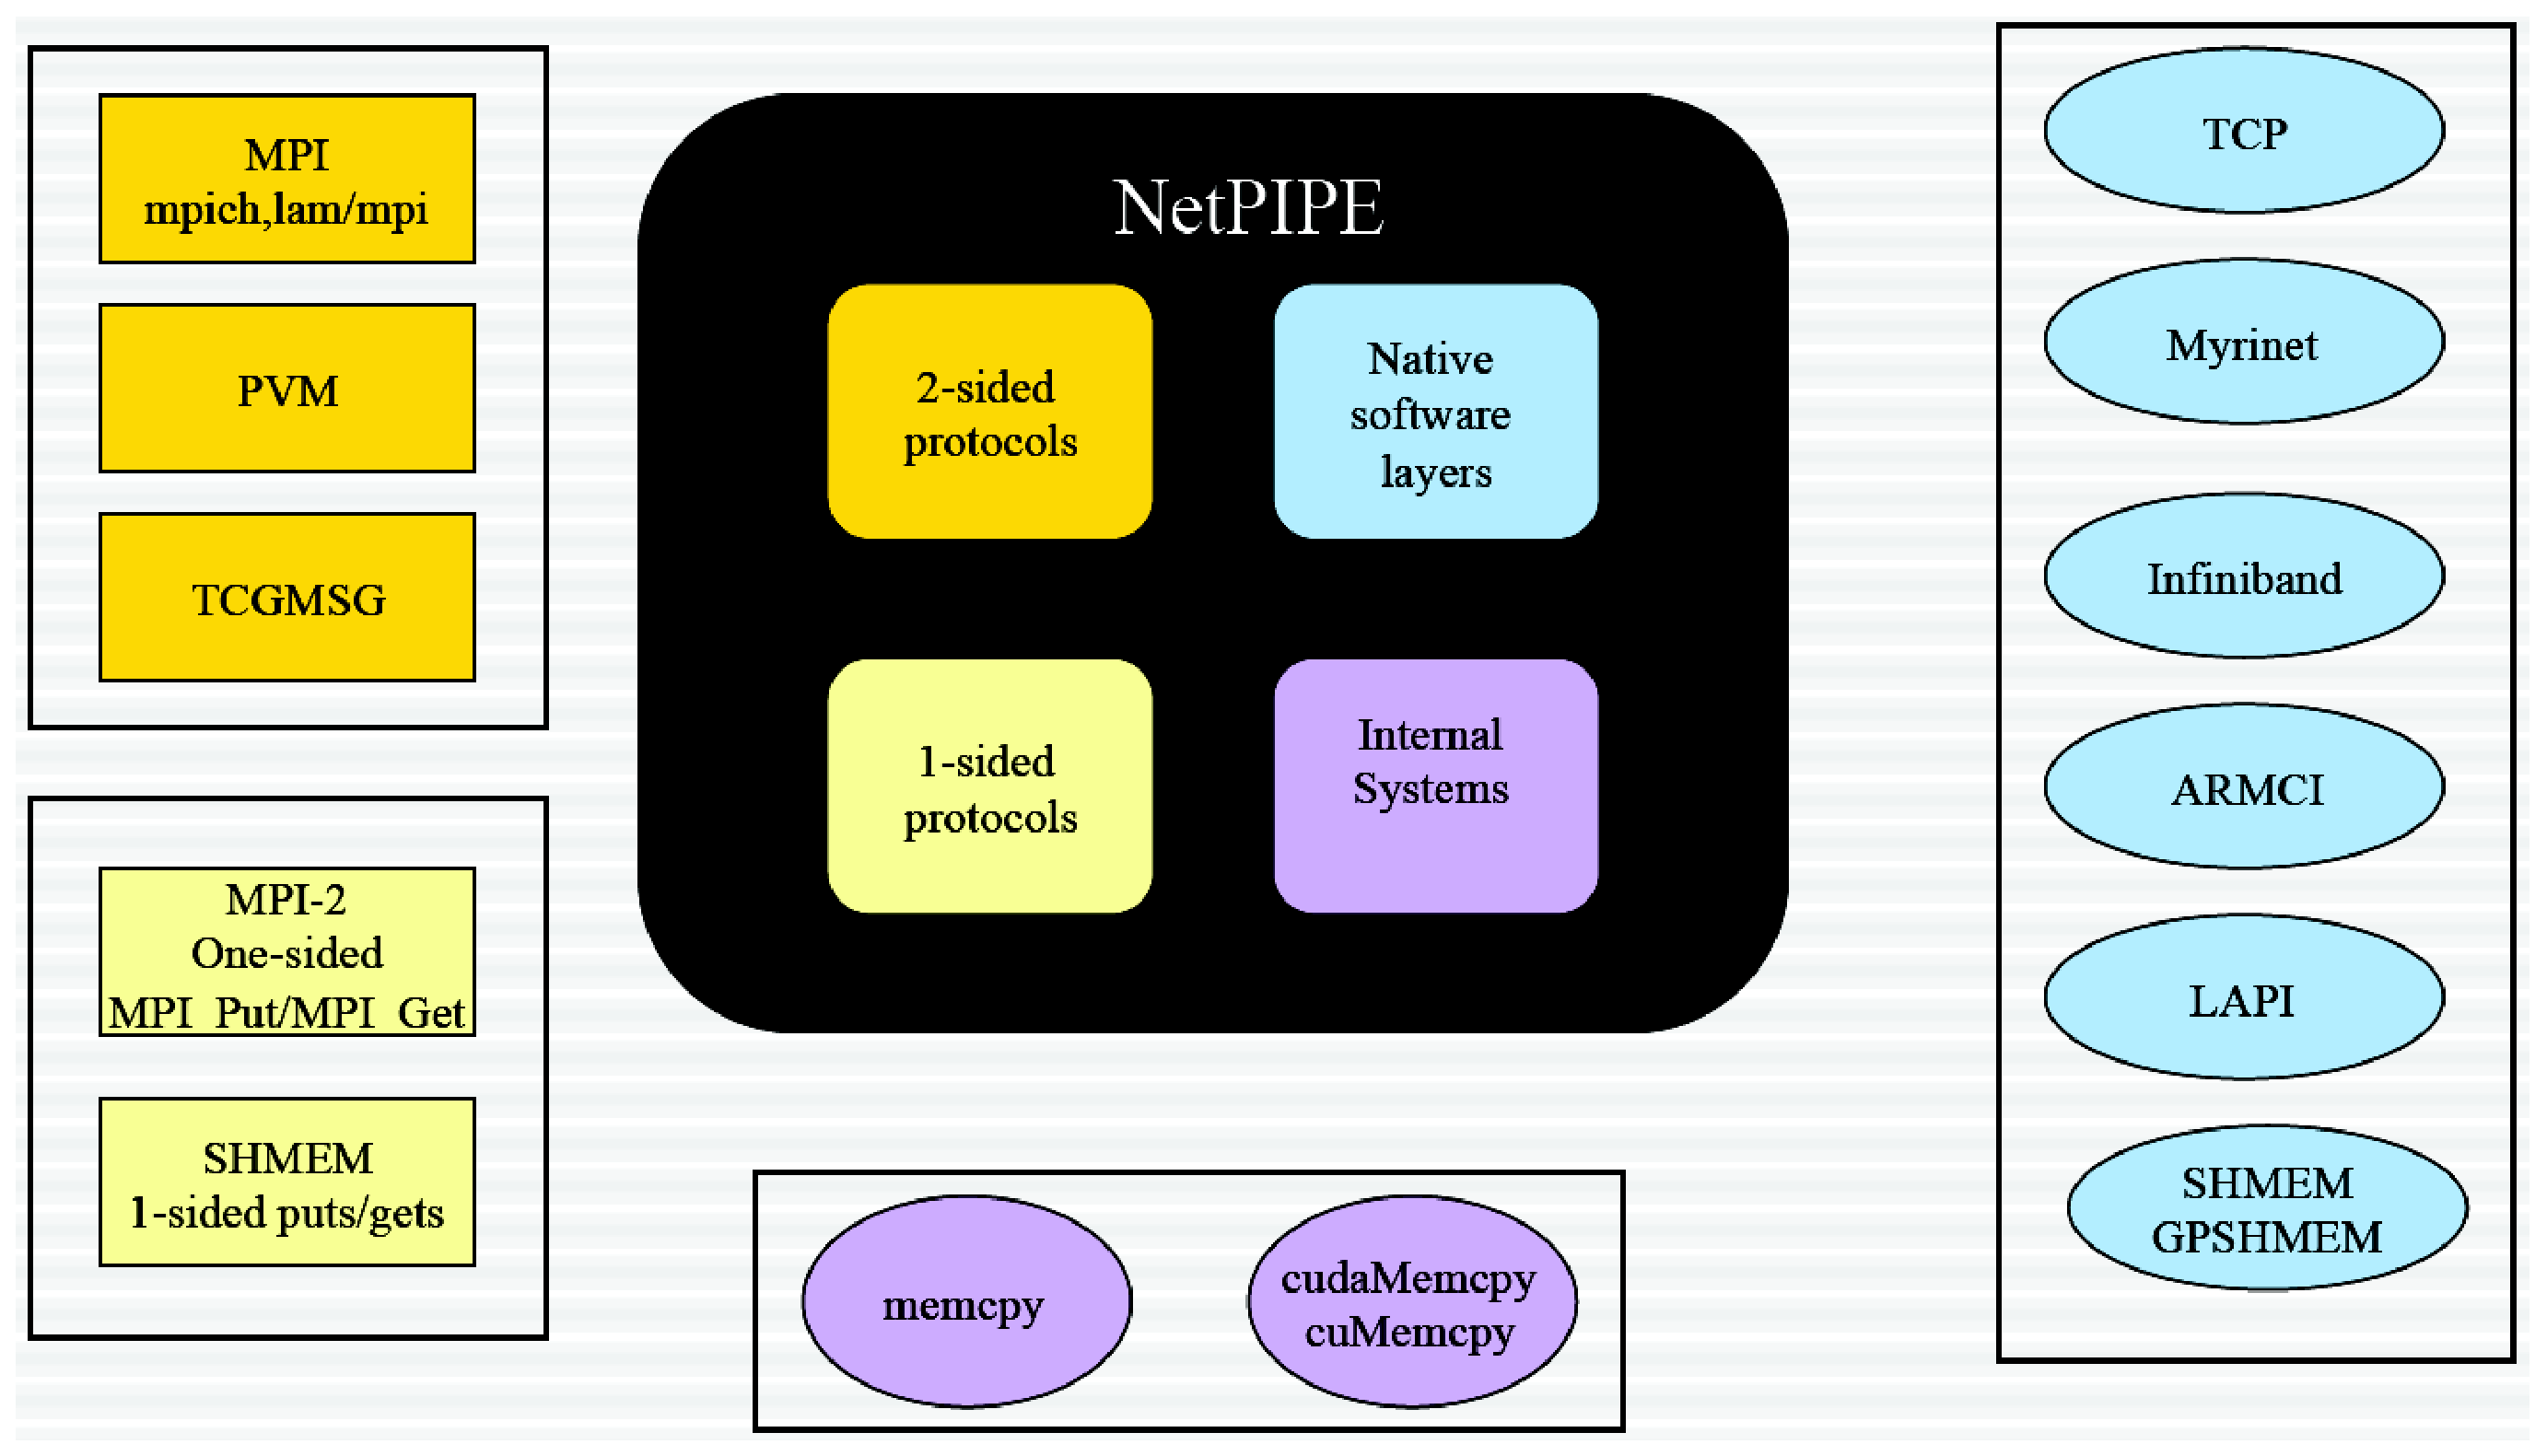
\includegraphics[height=5cm,
    angle=0]{./images/NetPIPE.eps}}
  \caption{NetPIPE}
  \label{fig:NetPIPE}
\end{figure}

NetPIPE allows us to measure and compare the performances at various
interconnect; thus allowing us to identify the bottleneck. Timing
measurements are done using \verb!gettimeofday()! system call.

NetPIPE provides the following subroutines
\begin{itemize}
\item \verb!NPcudaMemcpy!
\item \verb!NPcuMemcpy!
\end{itemize}


% NetPIPE Throughput plot
%  x-axis, packet size in Bytes in logarithmic scale
%  y-axis, throughput in Gigabits/sec
%  NetPIPE Latency plot
%  x-axis, packet size in Bytes in logarithmic scale
%  y-axix, latency in seconds in logarithmic scale

Benchmark system:
\begin{itemize}
\item Tesla S1070 system
\item Compute node = Dual Intel Core2 Quad Xeon 5405, 8 GB of main
  memory
\item Each compute node connect to 2 Tesla T10 via PCI-e 2.0 link.
\end{itemize}

\begin{itemize}
\item Paged memory is allocated via \verb!malloc()! function

\item Pinned (page-locked) memory is allocated via CUDA APIs. Memory
  in device is allocated as a linear array.
\end{itemize}
Memory transfers between the paged/page-locked (pinned) buffers on the
host and the device are studied
\begin{enumerate}
\item one-sided copies between host and the device
\item  roundtrip copies between host and the device
\item device to device memory copies
\end{enumerate}

\subsection{SGEMM/DGEMM CUBLAS}
\label{sec:sgemmdgemm-cublas}


Performance results of the GEMM routines from the CUBLAS library are
compared to that of the routines from the threaded implementation of
the Intel Math Kernel Library (MKL) BLAS routines. All the tests are
run on an Intel Xeon cluster equipped with NVIDIA Tesla S1070 GPUs.

SGEMM is 30\% slow on CUDA 3.0, it will be fixed in the next release
CUDA 3.1. 

